\documentclass[11pt]{article}

\usepackage[margin=1in]{geometry}
\usepackage{amsmath,amssymb,amsthm}
\usepackage{booktabs}
\usepackage{enumitem}
\usepackage{graphicx}
\usepackage{hyperref}

\newcommand{\vct}[1]{\mathbf{#1}}
\newcommand{\mat}[1]{\mathbf{#1}}

\graphicspath{{figures/}{hw2/figures/}}
\hypersetup{colorlinks=true,linkcolor=black,urlcolor=blue}

\title{EE 511 Homework 2\\[0.4em]
\large Information Theory, Discriminative Models, and Optimizers}
\author{Harshavardhan Reddy Narra}
\date{Fall 2026}

\begin{document}
\maketitle

\paragraph{Notation.}
Vectors are column vectors written in bold lowercase (\(\vct{x}\));
matrices are bold uppercase (\(\mat{W}\)).
\(\log_2\) measures information in bits and \(\ln\) in nats.
\(\vct{1}\) is the all-ones vector, \(\odot\) the element-wise product,
\(\mathbb{I}[\cdot]\) the indicator, and
\(\mathrm{softmax}(\vct{z})_k = e^{z_k}/\sum_j e^{z_j}\).
``MAC'' means one multiply--accumulate (\(=\ 2\) FLOPs).

\tableofcontents
\newpage

\section*{Part A: Theory}
\addcontentsline{toc}{section}{Part A: Theory}

%======================================================================
\section{Problem 1: Entropy, Divergence, and the Sampling Datapath}
%======================================================================

\subsection*{(a) Compression bound for a sparse stream}

An INT8 activation is exactly zero with probability \(s\), and otherwise
takes one of 64 nonzero codes, each equally likely. That is a
65-symbol alphabet with
\[
P(0)=s,
\qquad
P(\text{nonzero code }i)=\frac{1-s}{64}.
\]

\paragraph{(i) Entropy.}
\begin{align*}
H(s)
&= -s\log_2 s
   - 64\cdot\frac{1-s}{64}\log_2\frac{1-s}{64} \\
&= -s\log_2 s
   - (1-s)\bigl(\log_2(1-s)-\log_2 64\bigr) \\
&= -s\log_2 s-(1-s)\log_2(1-s)+6(1-s) \\
&= h_2(s)+6(1-s).
\end{align*}
At \(s=0.75\),
\[
h_2(0.75)
= -0.75\log_2 0.75-0.25\log_2 0.25
= 0.811278\ \text{bits},
\]
so \(H(0.75)=0.811278+1.5=2.311278\) bits/activation.
Raw INT8 is 8 bits, and Shannon says no lossless encoder can beat
\(H\) bits/symbol, so the largest compression ratio is
\[
\frac{8}{H(0.75)}=\frac{8}{2.311278}=3.461\times.
\]

\paragraph{(ii) Flag encoder.}
One flag bit on every activation plus 6 bits on each nonzero one:
\[
\mathbb{E}[\text{bits}]=1+6(1-s)=2.5
\quad\text{at }s=0.75.
\]
The gap to the bound is \(2.5-2.311278=0.1887\) bits/activation.
As \(s\to 1\) the expected length goes to 1, so the ratio is stuck at
\(8\times\). The ceiling is the 1-bit flag you still write for every
zero. Huffman cannot beat that either: it spends at least one bit on
every symbol, zeros included. Run-length encoding escapes the ceiling
because one codeword covers a whole run of zeros; as the stream becomes
all zeros the bits per activation go to 0.

%----------------------------------------------------------------------
\subsection*{(b) KL-guided clipping}

\(P=(0.60,0.25,0.10,0.05)\),
\(Q_{\max}=(0.425,0.425,0.10,0.05)\),
\(Q_{\mathrm{clip}}=(0.60,0.25,0.12,0.03)\).

\paragraph{(i)}
\[
D_{\mathrm{KL}}(P\Vert Q)=\sum_i p_i\log_2\frac{p_i}{q_i}.
\]
I get
\[
D_{\mathrm{KL}}(P\Vert Q_{\max})=0.10712\ \text{bits},
\qquad
D_{\mathrm{KL}}(P\Vert Q_{\mathrm{clip}})=0.01054\ \text{bits}.
\]
The entropy calibrator picks \(Q_{\mathrm{clip}}\). It wins by about
\(0.107/0.0105\approx 10.2\times\). Coding view: \(D_{\mathrm{KL}}(P\Vert Q)\)
is the extra bits you spend coding \(P\)-samples with a \(Q\)-code. The
outlier scale wastes \(\approx 0.107\) bits/sample by smearing the two
dense bins; the clipped scale only wastes \(\approx 0.011\).

\paragraph{(ii)}
\(Q_0=(0.60,0.25,0.15,0)\) puts zero mass on a bin that \(P\) actually
hits (\(p_4=0.05>0\)), so
\[
D_{\mathrm{KL}}(P\Vert Q_0)=\infty.
\]
A code that assigns probability 0 to a symbol that shows up has
infinite surprise. \(P\) is the reference (the real calibration
histogram); \(Q\) is the code induced by the scale. That is why the
order is \(P\Vert Q\) and not the other way around: we measure the
extra cost of coding the true stream. Infinite KL is what stops the
calibrator from clipping the tail all the way to zero. A tighter scale
would resolve the dense bins more finely, but one leftover sample in
the killed bin makes the code illegal.

%----------------------------------------------------------------------
\subsection*{(c) Correlation versus mutual information}

\paragraph{(i) Channel \(X\).}
\(X\in\{-1,0,+1\}\) with equal probability \(1/3\), and \(Y=X^2\).
Then \(Y=0\) iff \(X=0\) and \(Y=1\) otherwise, so
\(P(Y=1)=2/3\), \(P(Y=0)=1/3\).
\[
\mathbb{E}[X]=0,\qquad
\mathbb{E}[Y]=\tfrac23,\qquad
\mathbb{E}[XY]=\mathbb{E}[X^3]=0,
\]
hence \(\mathrm{Cov}(X,Y)=0\) and the Pearson correlation is exactly 0.
The pair \((X,Y)\) is a deterministic function of \(X\), so
\(H(X,Y)=H(X)=\log_2 3=1.5850\) bits.
\[
H(Y)=h_2(1/3)=0.9183\ \text{bits},
\qquad
I(X;Y)=H(X)+H(Y)-H(X,Y)=H(Y)=0.9183\ \text{bits}.
\]

\paragraph{(ii) Channel \(Z\).}
The given joint is already normalized. Marginals:
\[
P(Y=1)=\tfrac23,\quad
P(Z=1)=\tfrac{19}{30},\quad
\mathbb{E}[YZ]=\tfrac35.
\]
\[
\mathrm{Cov}(Z,Y)=\tfrac35-\tfrac23\cdot\tfrac{19}{30}=\tfrac{8}{45},
\qquad
r_{ZY}=\frac{8/45}{\sqrt{(2/9)(209/900)}}=0.7826.
\]
\[
H(Z)=0.9481,\quad
H(Y,Z)=1.3873,\quad
I(Z;Y)=H(Y)+H(Z)-H(Y,Z)=0.4791\ \text{bits}.
\]

\paragraph{(iii)}
A compiler that ranks by \(|r|\) keeps \(Z\) (\(0.78\) vs.\ \(0\)).
One that ranks by mutual information keeps \(X\) (\(0.918\) vs.\ \(0.479\)).
The slot should go to \(X\): \(Y\) is a deterministic function of \(X\),
so the channel tells you the label exactly. The bound
\(I\le\min\{H(\cdot),H(Y)\}\) is attained by \(X\)
(\(I(X;Y)=H(Y)\)); attaining it means one variable is a deterministic
function of the other. \(Z\) is well below the bound. Correlation missed
this because \(Y=X^2\) is an even map, so the linear association is zero
even though the information is complete.

%----------------------------------------------------------------------
\subsection*{(d) Temperature, truncation, and inverse-CDF sampling}

Logits \(\vct{z}=(\ln 8,\ln 4,\ln 2,0,0)\).

\paragraph{(i)}
At \(T=1\), \(\mathrm{softmax}(\vct{z})=(1/2,1/4,1/8,1/16,1/16)\) and
\[
H=1\cdot\tfrac12+2\cdot\tfrac14+3\cdot\tfrac18+4\cdot\tfrac{1}{16}+4\cdot\tfrac{1}{16}=1.875\ \text{bits}.
\]
\begin{center}
\begin{tabular}{c l c}
\toprule
\(T\) & \(\vct{p}_T\) & \(H\) (bits) \\
\midrule
\(1/2\) & \((64,16,4,1,1)/86\) & \(1.1239\) \\
\(1\)   & \((8,4,2,1,1)/16\)   & \(1.8750\) \\
\(2\)   & \((2\sqrt{2},2,\sqrt{2},1,1)/S\) & \(2.2000\) \\
\bottomrule
\end{tabular}
\end{center}
(\(S=2\sqrt{2}+2+\sqrt{2}+2\approx 8.2426\).)
Low \(T\) sharpens; high \(T\) flattens; entropy follows.

\paragraph{(ii)}
Top-\(p\) with \(p=0.8\) keeps the shortest prefix whose mass is at
least 0.8. That is 2 tokens at \(T=1/2\) (cdf \(0.744,0.930\)),
3 tokens at \(T=1\) (cdf \(0.50,0.75,0.875\)), and 4 tokens at
\(T=2\) (cdf \(0.343,0.586,0.757,0.879\)).
Top-\(k=2\) always keeps 2. So the two rules agree only at \(T=1/2\).
Top-\(k\) is a fixed-width sort: it maps onto a bitonic sorting
network of wired depth. Top-\(p\) has a data-dependent survivor
count, so the decoder has to allocate a variable buffer and the
threads diverge.

\paragraph{(iii)}
Full inverse-CDF at \(T=1\), \(U=0.8\): the cdf is
\((0.50,0.75,0.875,0.9375,1)\), so \(U\) lands in
\((0.75,0.875]\) and we emit token 3.
After top-\(p=0.8\) we keep the first three and renormalize to
\((4/7,2/7,1/7)\). The new cdf is \((0.571,0.857,1)\), so the same
\(U=0.8\) now lands in \((0.571,0.857]\) and we emit token 2.
The two procedures do \emph{not} emit the same token.
Truncation + renormalize rewrites the cdf, so a leftover uniform
draw can jump to a different atom.

\paragraph{(iv)}
Varentropy of the \(T=1\) distribution, in bits\(^2\):
\[
V=\mathbb{E}[(\log_2 p)^2]-(\mathbb{E}[\log_2 p])^2
=4.625-(1.875)^2=1.109375.
\]
\(V=0\) iff \(-\log p\) is a.s.\ constant, i.e.\ the distribution is
a point mass (or uniform over a subset of equal probabilities --- but
a one-hot is the clean case the slide cares about). A sudden spike in
\(V\) means the model just became multi-modal / high-uncertainty; the
gating controller on [M2:106] would kick the decode onto a heavier
path (more samples, higher precision, or a speculative branch) instead
of treating the step as a confident argmax.

%----------------------------------------------------------------------
\subsection*{(e) Single-pass softmax}

\paragraph{(i)}
Keep a running max \(m_k\) and a running sum \(S_k\) over the first
\(k\) logits. For a new logit \(x_{k+1}\):
\[
\begin{aligned}
m_{k+1}&=\max(m_k,x_{k+1}),\\
S_{k+1}
&=
\begin{cases}
S_k+e^{x_{k+1}-m_k}
  & \text{if }x_{k+1}\le m_k,\\[2pt]
S_k\,e^{m_k-x_{k+1}}+1
  & \text{if }x_{k+1}>m_k.
\end{cases}
\end{aligned}
\]
When the max moves, every old term was computed against \(m_k\) and
must be rescaled by the single factor \(e^{m_k-m_{k+1}}\).
Claim: \(S_k=\sum_{j\le k}e^{x_j-m_k}\) after every step.
Base: \(S_1=1=e^{x_1-x_1}\).
Inductive step, case \(x_{k+1}\le m_k\): add \(e^{x_{k+1}-m_k}\) and
the max does not move.
Case \(x_{k+1}>m_k\):
\[
S_{k+1}
=S_k e^{m_k-x_{k+1}}+1
=\sum_{j\le k}e^{x_j-x_{k+1}}+e^{x_{k+1}-x_{k+1}}
=\sum_{j\le k+1}e^{x_j-m_{k+1}}.
\]

\paragraph{(ii)}
On \(\vct{x}=(2,5,1,6)\), to four decimals:
\begin{center}
\begin{tabular}{c cc}
\toprule
\(k\) & \(m_k\) & \(S_k\) \\
\midrule
1 & 2 & 1.0000 \\
2 & 5 & 1.0498 \\
3 & 5 & 1.0681 \\
4 & 6 & 1.3929 \\
\bottomrule
\end{tabular}
\end{center}
Softmax:
\[
\vct{p}
=\frac{(e^{2-6},e^{5-6},e^{1-6},e^{6-6})}{1.3929}
=(0.01315,\,0.26410,\,0.00484,\,0.71791).
\]

\paragraph{(iii)}
Every exponential the recurrence evaluates is either
\(e^{x_{k+1}-m_k}\) with \(x_{k+1}\le m_k\), or
\(e^{m_k-x_{k+1}}\) with \(x_{k+1}>m_k\), or \(e^0=1\).
The argument is always \(\le 0\), so the result is in \((0,1]\) and
cannot overflow even in FP8 E4M3 (overflow beyond \(\approx 6.1\)).
Max-shifted softmax does a max pass and then a sum pass, i.e.\ two
full reads of the logit vector. The online version fuses them.
For a 32{,}000-token vocabulary in FP16 that saves
\[
32\,000\times 2\ \text{B}=64\ \text{KB}
\]
of logit traffic per generated token.

%======================================================================
\section{Problem 2: Backpropagation, Losses, and the Optimizer Memory Wall}
%======================================================================

\subsection*{(a) The softmax Jacobian}

From the two cases on [M2:122],
\(\partial p_i/\partial z_j=p_i(\delta_{ij}-p_j)\), which is exactly
\[
\mat{J}=\frac{\partial\vct{p}}{\partial\vct{z}}=\mathrm{diag}(\vct{p})-\vct{p}\vct{p}^\top.
\]
\(\mat{J}^\top=\mat{J}\) because \(\mathrm{diag}(\vct{p})\) and
\(\vct{p}\vct{p}^\top\) are symmetric.
\[
\mat{J}\vct{1}
=\vct{p}-\vct{p}(\vct{p}^\top\vct{1})
=\vct{p}-\vct{p}=\vct{0},
\]
since \(\vct{p}\) already sums to 1. That is the infinitesimal form of
shift invariance: \(\mathrm{softmax}(\vct{z}+c\vct{1})=\mathrm{softmax}(\vct{z})\)
for every \(c\), so the directional derivative along \(\vct{1}\) is zero.
For \(\vct{p}=(0.5,0.3,0.2)\),
\[
\mat{J}
=
\begin{pmatrix}
0.25 & -0.15 & -0.10 \\
-0.15 & 0.21 & -0.06 \\
-0.10 & -0.06 & 0.16
\end{pmatrix}.
\]

%----------------------------------------------------------------------
\subsection*{(b) Hinge loss}

Scores \(\vct{s}=(2.0,1.5,-0.5,2.3)\), correct class is class 1
(1-indexed, so \(s_y=2.0\)), \(\Delta=1\).
\[
L=\sum_{j\neq y}\max(0,s_j-s_y+\Delta)
=\max(0,0.5)+\max(0,-1.5)+\max(0,1.3)
=1.8.
\]
Regimes for the three incorrect classes:
class 2 is in the \emph{warning} band (\(s_2<s_y\) but the margin is
violated), class 3 is \emph{safe} (margin satisfied), class 4 is a
\emph{failure} (\(s_4>s_y\)).
\[
\frac{\partial L}{\partial\vct{s}}=(-2,\,1,\,0,\,1).
\]
One entry is exactly zero (the safe class). Hardware can skip that
class in the update --- no MAC, no write [M3:23].
The slide's ``0, \(-1\), or \(+1\)'' description is the
\emph{per-incorrect-class} contribution. The correct-class entry is
minus the number of violators, so it is an integer in
\(\{0,-1,\ldots,-(C-1)\}\). Here two classes violate, so we get \(-2\),
not \(-1\).

%----------------------------------------------------------------------
\subsection*{(c) Backpropagation by hand}

\paragraph{(i) Forward.}
\[
\vct{z}_1
=\mat{W}_1\vct{x}+\vct{b}_1
=
\begin{pmatrix}-0.5\\1.5\\0.5\end{pmatrix},
\qquad
\vct{h}=\max(\vct{0},\vct{z}_1)
=
\begin{pmatrix}0\\1.5\\0.5\end{pmatrix},
\]
\[
\vct{s}=\mat{W}_2\vct{h}+\vct{b}_2
=
\begin{pmatrix}1\\1\end{pmatrix},
\qquad
\vct{p}=\mathrm{softmax}(\vct{s})
=
\begin{pmatrix}0.5\\0.5\end{pmatrix},
\qquad
L=-\ln p_1=\ln 2=0.693147.
\]

\paragraph{(ii) Backward (shapes in parentheses).}
\[
\frac{\partial L}{\partial\vct{s}}=\vct{p}-\vct{y}
=
\begin{pmatrix}-0.5\\0.5\end{pmatrix}\ (2),
\qquad
\frac{\partial L}{\partial\mat{W}_2}
=\frac{\partial L}{\partial\vct{s}}\,\vct{h}^\top
=
\begin{pmatrix}
0 & -0.75 & -0.25 \\
0 &  0.75 &  0.25
\end{pmatrix}\ (2\times 3),
\]
\[
\frac{\partial L}{\partial\vct{b}_2}
=\frac{\partial L}{\partial\vct{s}}\ (2),
\qquad
\frac{\partial L}{\partial\vct{h}}
=\mat{W}_2^\top\frac{\partial L}{\partial\vct{s}}
=
\begin{pmatrix}-1\\0.5\\-1\end{pmatrix}\ (3),
\]
\[
\frac{\partial L}{\partial\vct{z}_1}
=\frac{\partial L}{\partial\vct{h}}\odot\mathbb{I}[\vct{z}_1>0]
=
\begin{pmatrix}0\\0.5\\-1\end{pmatrix}\ (3),
\]
\[
\frac{\partial L}{\partial\mat{W}_1}
=\frac{\partial L}{\partial\vct{z}_1}\,\vct{x}^\top
=
\begin{pmatrix}
0 & 0 \\
0.5 & 1 \\
-1 & -2
\end{pmatrix}\ (3\times 2),
\qquad
\frac{\partial L}{\partial\vct{b}_1}
=\frac{\partial L}{\partial\vct{z}_1}\ (3).
\]

\paragraph{(iii) Exact zeros.}
All of column 1 of \(\partial L/\partial\mat{W}_2\) is zero because
\(h_1=0\) (ReLU killed the first hidden unit, so that incoming weight
was never used). The entire first row of \(\partial L/\partial\mat{W}_1\)
is zero because \(\partial L/\partial z_{1,1}=0\) (same ReLU mask).
Tensors that have to be stashed for the backward pass:
\(\vct{x}\) (for \(d\mat{W}_1\)), \(\vct{h}\) (for \(d\mat{W}_2\)),
and the ReLU mask \(\mathbb{I}[\vct{z}_1>0]\) (for the VJP through
ReLU). The mask is 1 bit/element [M3:59, M3:68]. \(\mat{W}_2\) is also
needed for \(\partial L/\partial\vct{h}\), but that is a parameter, not
an activation.

\paragraph{(iv) One SGD step, \(\eta=0.1\).}
\[
\mat{W}_2\leftarrow
\begin{pmatrix}1 & 0.075 & 2.025\\ -1 & 0.925 & -0.025\end{pmatrix},
\quad
\vct{b}_2\leftarrow
\begin{pmatrix}0.05\\ -0.55\end{pmatrix},
\]
\[
\mat{W}_1\leftarrow
\begin{pmatrix}1 & -1\\ 0.45 & 0.4\\ -0.9 & 1.2\end{pmatrix},
\quad
\vct{b}_1\leftarrow
\begin{pmatrix}0.5\\ -0.05\\ -0.4\end{pmatrix}.
\]
Rerun:
\(\vct{z}_1=(-0.5,1.2,1.1)^\top\),
\(\vct{h}=(0,1.2,1.1)^\top\),
\(\vct{s}=(2.3675,0.5325)^\top\),
\(p_1=0.8624\),
new loss \(L=0.1481\). It dropped, as it should.

%----------------------------------------------------------------------
\subsection*{(d) What Adam's normalization buys}

\paragraph{(i)}
At \(t=1\), \(m_0=v_0=0\), so
\(m_1=(1-\beta_1)g_1\), \(v_1=(1-\beta_2)g_1^2\).
Bias correction undoes both factors:
\(\hat m_1=g_1\), \(\hat v_1=g_1^2\).
The step is
\[
w_1-w_0
=-\eta\frac{\hat m_1}{\sqrt{\hat v_1}+\epsilon}
=-\eta\,\mathrm{sign}(g_1)
\]
for any \(g_1\neq 0\). Magnitude drops out; the first step is just
\(\pm\eta\). That matches the walkthrough on [M3:87]--[M3:90].

\paragraph{(ii)}
Without bias correction the first step is
\[
-\eta\frac{(1-\beta_1)g_1}{\sqrt{(1-\beta_2)g_1^2}}
=-\eta\frac{1-\beta_1}{\sqrt{1-\beta_2}}\,\mathrm{sign}(g_1)
=-\eta\cdot\frac{0.1}{\sqrt{0.001}}\,\mathrm{sign}(g_1)
=-3.162\,\eta\,\mathrm{sign}(g_1).
\]
Too \emph{large}, not too small. ``Biased toward zero'' is true of
both \(m\) and \(v\), but \(v\) is more biased (\(\beta_2=0.999\) vs.\
\(\beta_1=0.9\)), so \(\sqrt{v}\) is tiny and the ratio \(m/\sqrt{v}\)
blows up. Bias correction exists to kill that first-step spike.

\paragraph{(iii)}
If every gradient is multiplied by \(c>0\):
SGD scales by \(c\) (need to retune \(\eta\));
momentum \(v\leftarrow\rho v+\eta g\) also scales by \(c\) (retune
\(\eta\));
Adam's \(m\) and \(\sqrt{v}\) both scale by \(c\), so the ratio is
unchanged. Only SGD and momentum need a new learning rate.

%----------------------------------------------------------------------
\subsection*{(e) The optimizer memory wall}

\(N=1.3\times 10^9\) parameters, \(1\,\mathrm{GB}=10^9\) bytes.

\paragraph{(i) Static footprint (weights + gradients + optimizer state).}
I used the usual mixed-precision Adam packing: FP16 weight copy,
FP16 gradient, FP32 master weight, plus FP32 \(m\) and \(v\).
INT8 \(m,v\) add one FP32 scale per block of 256 for each of \(m\) and
\(v\), i.e.\ \(8/256=0.03125\) B/param of metadata.
\begin{center}
\begin{tabular}{lcc}
\toprule
Configuration & B/param & Footprint (GB) \\
\midrule
FP32 SGD & 8 & 10.40 \\
FP32 SGD + momentum & 12 & 15.60 \\
FP32 Adam & 16 & 20.80 \\
Mixed-precision Adam & 16 & 20.80 \\
Mixed-precision Adam, INT8 \(m,v\) & 10.03125 & 13.04 \\
\bottomrule
\end{tabular}
\end{center}
Mixed-precision Adam does \emph{not} shrink the optimizer state; it
just adds an FP16 working copy. The 4-byte \(m\) and \(v\) are still
there.

\paragraph{(ii)}
Activations add 4 to 8 B/param, i.e.\ 5.2 to 10.4 GB.
Mixed-precision Adam: \(20.8+5.2=26.0>24\) already, and
\(31.2\) GB at the high end. It does not fit anywhere in that range.
INT8 states: \(13.04+5.2=18.24\) GB and \(13.04+10.4=23.44\) GB. Both
ends fit in 24 GB.

\paragraph{(iii)}
Bandwidth \(2.0\) TB/s \(=2\times 10^{12}\) B/s.
Per-parameter traffic, FP32 states: read FP16 \(g\) (2),
read+write master / \(m\) / \(v\) (8+8+8), write FP16 weight (2)
\(=28\) B.
INT8 states: 2 + 8 + 2 + 2 + 2 + scale traffic
\(2\times(8/256)=0.0625\), total \(16.0625\) B.
\[
t_{\mathrm{FP32}}=\frac{1.3\times10^9\cdot 28}{2\times10^{12}}=18.2\ \mathrm{ms},
\qquad
t_{\mathrm{INT8}}=10.44\ \mathrm{ms}.
\]
States shrink \(4\times\) but they were only 16 of the 28 bytes. The
master weight and the FP16 copies do not shrink, so the step speeds up
by \(28/16.06\approx 1.74\times\), nowhere near \(4\times\).

\newpage
\section*{Part B: Programming}
\addcontentsline{toc}{section}{Part B: Programming}

\paragraph{Compute environment.}
Seed 511, NumPy 2.4.6, local CPU, 32 cores.
No autograd in Problems 3 or 4 (torchvision is used only to download
the datasets). Every number below comes from \texttt{problem3.py} and
\texttt{problem4.py}.

%======================================================================
\section{Problem 3: Linear Classifiers on CIFAR-10, from Scratch}
%======================================================================

Setup as specified: 45{,}000 / 5{,}000 train/val split at seed 511,
flatten to \(D=3072\), z-score from the training split only, bias trick
so \(\widetilde{\mat{W}}\in\mathbb{R}^{10\times 3073}\), scores
\(\mat{S}=\mat{X}\widetilde{\mat{W}}^\top\), init
\(\mathcal{N}(0,10^{-6})\), minibatch SGD with \(B=256\), 20 epochs.

% numbers filled after the run
\subsection*{(a) Losses and gradients}

Both losses and both gradients are fully vectorized in
\texttt{problem3.py}. L2 is \(\frac12\sum W_{ij}^2\) on the weight
columns and not the bias column.

Centered finite-difference check, \(h=10^{-5}\), float64, batch of 32,
10 random coordinates:
\begin{center}
\begin{tabular}{lc}
\toprule
Loss & max relative error \\
\midrule
SVM & \(3.99\times 10^{-10}\) \\
softmax & \(1.36\times 10^{-9}\) \\
\bottomrule
\end{tabular}
\end{center}
Both are well under \(10^{-7}\). An occasional large SVM error is still
possible in principle: the hinge \(\max(0,s_j-s_y+\Delta)\) is not
differentiable on the kink, so a centered difference that straddles a
kink can disagree with the 0-subgradient we return there. None of my
10 SVM coordinates hit that case. A full centered-difference gradient
on \(\widetilde{\mat{W}}\) needs \(2\times 10\times 3073=61{,}460\)
forward passes. Backprop needs one forward and one backward [M3:74].

\subsection*{(b) Training and tuning}

Validation-accuracy grids (best epoch on the 5k split):

\paragraph{Softmax (val acc).}
\begin{center}
\begin{tabular}{lccc}
\toprule
\(\eta \backslash \lambda\) & \(10^{-2}\) & \(10^{-1}\) & \(1\) \\
\midrule
\(10^{-2}\) & \textbf{0.4160} & 0.4116 & 0.3848 \\
\(10^{-3}\) & 0.4144 & 0.4128 & 0.3986 \\
\(10^{-4}\) & 0.3778 & 0.3772 & 0.3686 \\
\bottomrule
\end{tabular}
\end{center}

\paragraph{SVM (val acc).}
\begin{center}
\begin{tabular}{lccc}
\toprule
\(\eta \backslash \lambda\) & \(10^{-2}\) & \(10^{-1}\) & \(1\) \\
\midrule
\(10^{-3}\) & 0.4048 & 0.4046 & 0.3986 \\
\(3\times 10^{-4}\) & \textbf{0.4066} & 0.4054 & 0.4022 \\
\(10^{-4}\) & 0.3980 & 0.3962 & 0.3964 \\
\bottomrule
\end{tabular}
\end{center}

Best softmax: \(\eta=10^{-2}\), \(\lambda=10^{-2}\), test accuracy
\(0.4006\). Best SVM: \(\eta=3\times 10^{-4}\), \(\lambda=10^{-2}\),
test accuracy \(0.3961\). Both land in the 35--42\% band the
assignment asked for.

\begin{figure}[ht]
\centering
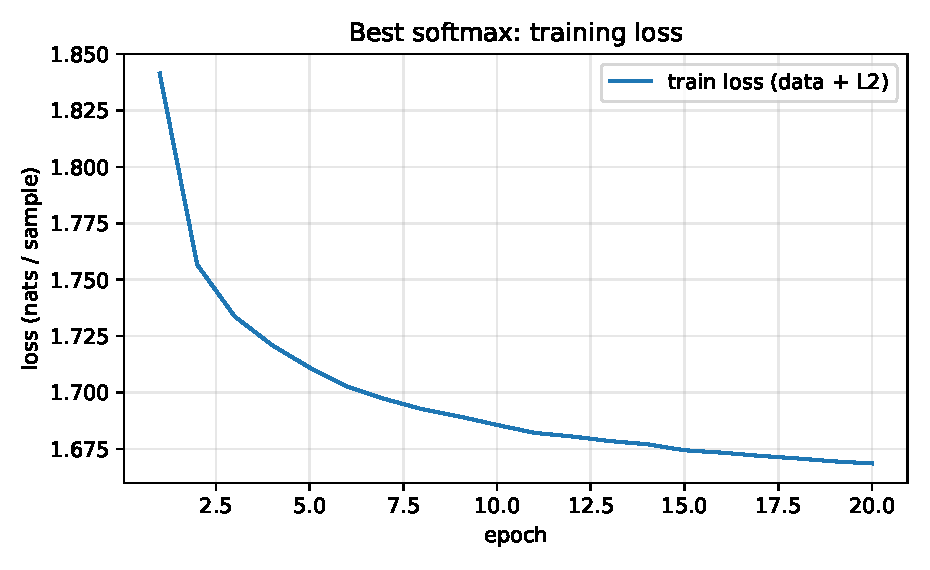
\includegraphics[width=0.48\textwidth]{p3_softmax_loss.pdf}
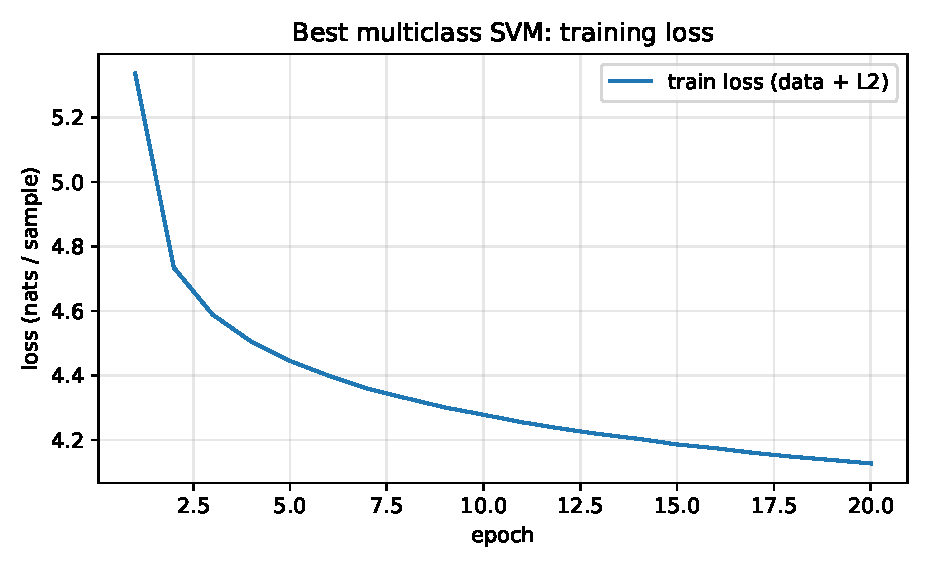
\includegraphics[width=0.48\textwidth]{p3_svm_loss.pdf}
\caption{Training loss vs.\ epoch for the validation-best softmax
(left) and SVM (right). Loss is nats (softmax) or hinge units (SVM)
per sample, including the L2 term.}
\end{figure}

L2 does \emph{not} help here. The best softmax ends at train / val /
test \(0.443/0.411/0.401\); the best SVM at \(0.414/0.407/0.396\).
The train--val gap is only about 3 points. Turning \(\lambda\) up to
1.0 drops softmax val from 0.416 to 0.385 and SVM val from 0.407 to
0.402, and the training accuracy falls with it. A linear model cannot
overfit 45k CIFAR images with one template per class [M3:34], so the
regularizer is just shrinking a model that is already underfitting.

\subsection*{(c) Templates}

\begin{figure}[ht]
\centering
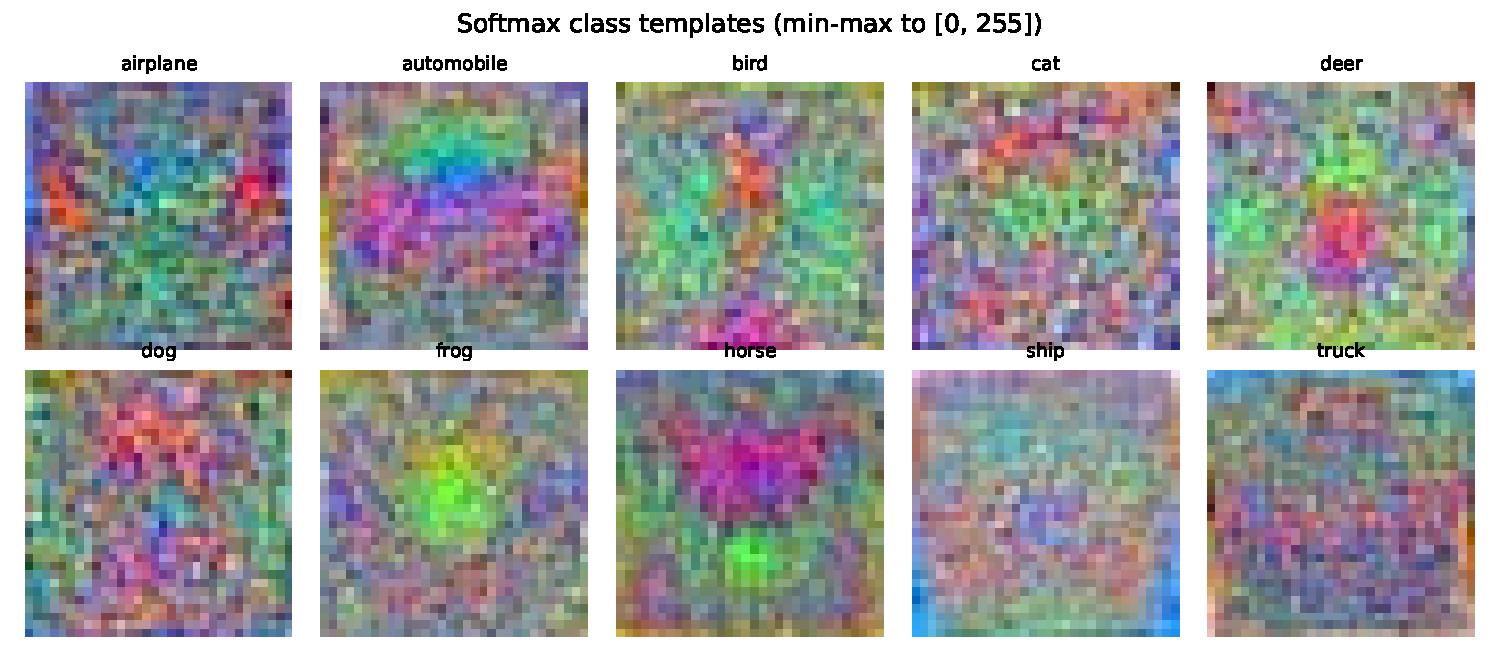
\includegraphics[width=0.95\textwidth]{p3_softmax_templates.pdf}
\caption{Softmax class templates, each \(32\times 32\times 3\) weight
row min-max rescaled to \([0,255]\).}
\end{figure}

\begin{figure}[ht]
\centering
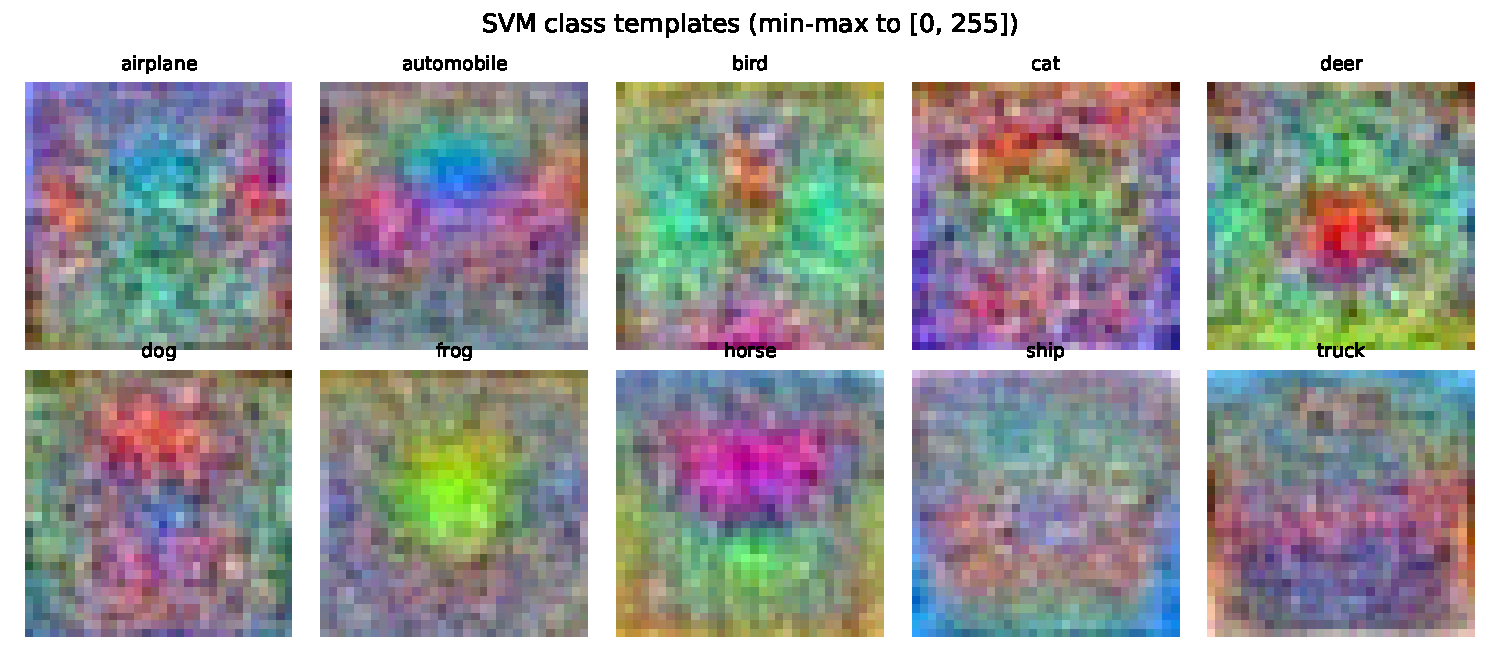
\includegraphics[width=0.95\textwidth]{p3_svm_templates.pdf}
\caption{SVM class templates, same unflatten and rescale.}
\end{figure}

A single linear template per class has to average every pose, color,
and subclass of that class [M3:17]. Horse and bird are the clearest
failures: both are muddy purple/green blobs with no head, legs, or
wings. Cat and dog look the same way. The model is averaging
left-facing and right-facing animals, different breeds, and different
backgrounds into one image, so nothing coherent survives. Frog and
automobile do a little better (a green blob, a reddish car-ish blob)
only because those classes are more color-consistent. That is the
ceiling of a one-template model: it can lock onto a class-level color
prior, not onto an object. SVM templates look essentially the same,
which matches the almost-identical test accuracies.

\subsection*{(d) L1 versus L2}

Softmax retrained at \(\eta=10^{-3}\) with proximal soft-thresholding
on the weight columns after every step.
\begin{center}
\begin{tabular}{lccc}
\toprule
Penalty & test acc & exactly-zero weights \\
\midrule
L2 (best, \(\lambda=10^{-2}\)) & 0.4006 & 0.00\% \\
L1 \(\lambda=10^{-3}\) & 0.4029 & 0.44\% \\
L1 \(\lambda=10^{-2}\) & 0.3461 & 19.88\% \\
L1 \(\lambda=3\times 10^{-2}\) & 0.2678 & 67.66\% \\
\bottomrule
\end{tabular}
\end{center}

\begin{figure}[ht]
\centering
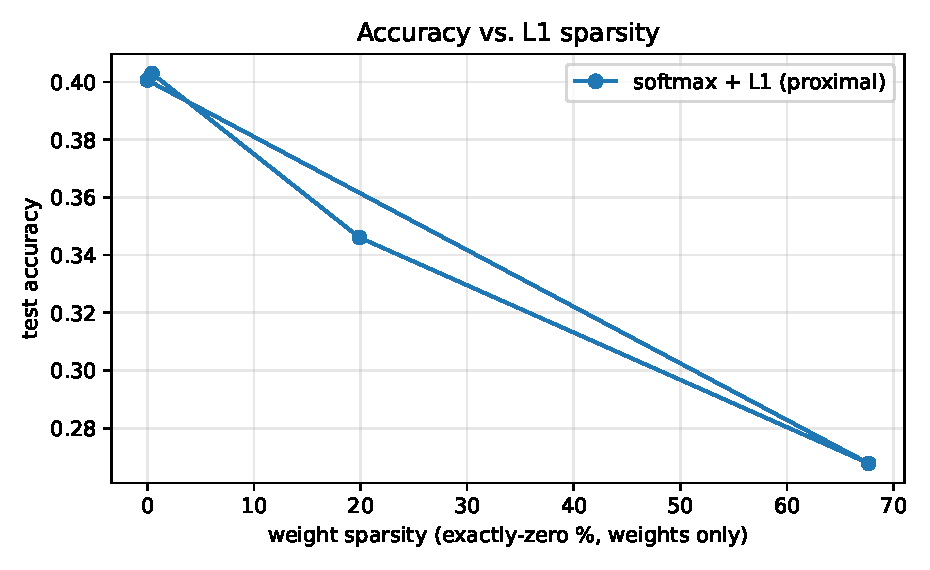
\includegraphics[width=0.7\textwidth]{p3_l1_sparsity.pdf}
\caption{Test accuracy vs.\ the percentage of exactly-zero weights
under L1 proximal SGD. L2 of the best softmax model sits at 0\%
sparsity.}
\end{figure}

L2 never produces exact zeros. L1 does, and past a point you are
deleting coordinates the linear model actually uses, so accuracy
falls [M3:34].

\subsection*{(e) Numerics and gradient sparsity}

\paragraph{(i)}
Naive \(\mathrm{softmax}\) in float16 on \((8,9,10)\) still returns a
finite vector. On \((10,11,12)\) it overflows
(\(\exp(12)\) in float16 is \(\infty\)), so the result is NaN.
Max-shifted softmax is finite on both.
The smallest input at which \(\mathtt{np.exp}\) overflows in float16
is \(11.09\) (analytic ceiling \(\ln 65504\approx 11.09\), matching
[M3:28]). Naive float16 softmax on \((8,9,10)\) is still finite,
\((0.090,0.245,0.665)\); on \((10,11,12)\) it returns
\((0,0,\mathrm{NaN})\) because \(\exp(12)\) overflows. Max-shifted
softmax is finite on both and matches the float64 answer to about
three digits.

\paragraph{(ii)}
\begin{figure}[ht]
\centering
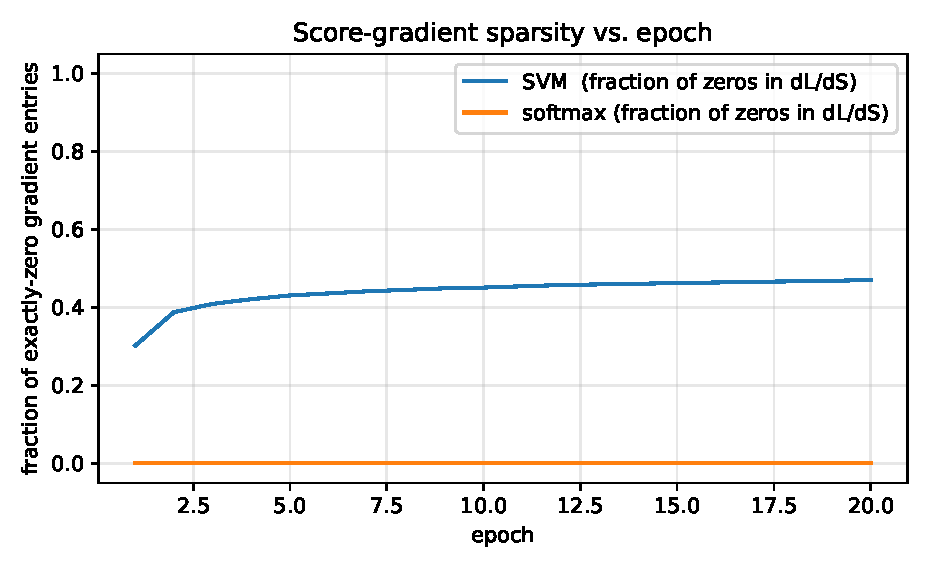
\includegraphics[width=0.7\textwidth]{p3_grad_sparsity.pdf}
\caption{Fraction of exactly-zero entries of \(\partial L/\partial S\),
averaged over each epoch.}
\end{figure}
SVM starts at 30\% exact zeros in \(\partial L/\partial S\) and climbs
to 47\% by epoch 20: as the scores separate, more incorrect classes
fall into the safe region and drop out of the gradient [M3:23].
Softmax's \(\mat{P}-\mat{Y}\) is never exact zero [M3:31], so that
curve sits on the axis for all 20 epochs.

\paragraph{(iii)}
\(10\times 3073=30{,}730\) parameters, FP32 footprint
\(30{,}730\times 4/1024=120.0\) KiB. It just fits in 128 KiB of
on-chip SRAM [M3:4].

%======================================================================
\section{Problem 4: An MLP and Five Optimizers, from Scratch}
%======================================================================

Fashion-MNIST, 54{,}000 / 6{,}000 split at seed 511, pixels to
\([0,1]\), then one scalar train mean/std.
Network \(784\to 512\to 256\to 10\), ReLU, softmax cross-entropy in
log-sum-exp form, He init, \(B=128\), 15 epochs, no regularization.

\subsection*{(a) Implementation and static analysis}

\paragraph{(i)}
Centered FD, float64, batch of 8, 10 random entries of each of the
six tensors. Every max relative error is under \(2\times 10^{-7}\).
\begin{center}
\begin{tabular}{lc}
\toprule
Tensor & max relative error \\
\midrule
\(\mat{W}_1\) & \(1.19\times 10^{-7}\) \\
\(\vct{b}_1\) & \(1.20\times 10^{-8}\) \\
\(\mat{W}_2\) & \(4.72\times 10^{-8}\) \\
\(\vct{b}_2\) & \(2.59\times 10^{-9}\) \\
\(\mat{W}_3\) & \(5.31\times 10^{-8}\) \\
\(\vct{b}_3\) & \(1.21\times 10^{-9}\) \\
\bottomrule
\end{tabular}
\end{center}

\paragraph{(ii)}
{\small
\begin{center}
\begin{tabular}{lrrlll}
\toprule
Layer & \#params & fwd MACs/sample & fwd \(XW\) & \(X^\top\delta\) & \(\delta W^\top\) \\
\midrule
\(784\to 512\) & 401{,}920 & 401{,}408 & \(128\times 784\times 512\) & \(784\times 128\times 512\) & \(128\times 512\times 784\) \\
\(512\to 256\) & 131{,}328 & 131{,}072 & \(128\times 512\times 256\) & \(512\times 128\times 256\) & \(128\times 256\times 512\) \\
\(256\to 10\)  & 2{,}570   & 2{,}560   & \(128\times 256\times 10\)  & \(256\times 128\times 10\)  & \(128\times 10\times 256\) \\
\midrule
Total & 535{,}818 & 535{,}040 & & & \\
\bottomrule
\end{tabular}
\end{center}
}
The first layer can skip \(\delta W^\top\) entirely: that GEMM is
\(\partial L/\partial X\), and the input image is not a parameter.

\paragraph{(iii)}
First layer does \(401{,}408/535{,}040=75.0\%\) of the forward MACs.
That is the computational asymmetry of [M3:49]: the wide first matmul
is where a systolic array and where quantization buy the most.

\subsection*{(b) Five optimizers}

Every run started from the same He initialization. All five beat 87\%
test accuracy.
\begin{center}
\begin{tabular}{lcccc}
\toprule
Optimizer & best \(\eta\) & best val acc & test acc & iters to 87\% val \\
\midrule
SGD & \(0.1\) & 0.8975 & 0.8856 & 875 \\
momentum & \(0.03\) & 0.8975 & 0.8913 & 425 \\
AdaGrad & \(0.01\) & 0.8970 & 0.8869 & 650 \\
RMSProp & \(3\times 10^{-4}\) & 0.8983 & 0.8796 & 675 \\
Adam & \(3\times 10^{-4}\) & 0.8972 & 0.8930 & 600 \\
\bottomrule
\end{tabular}
\end{center}

\begin{figure}[ht]
\centering
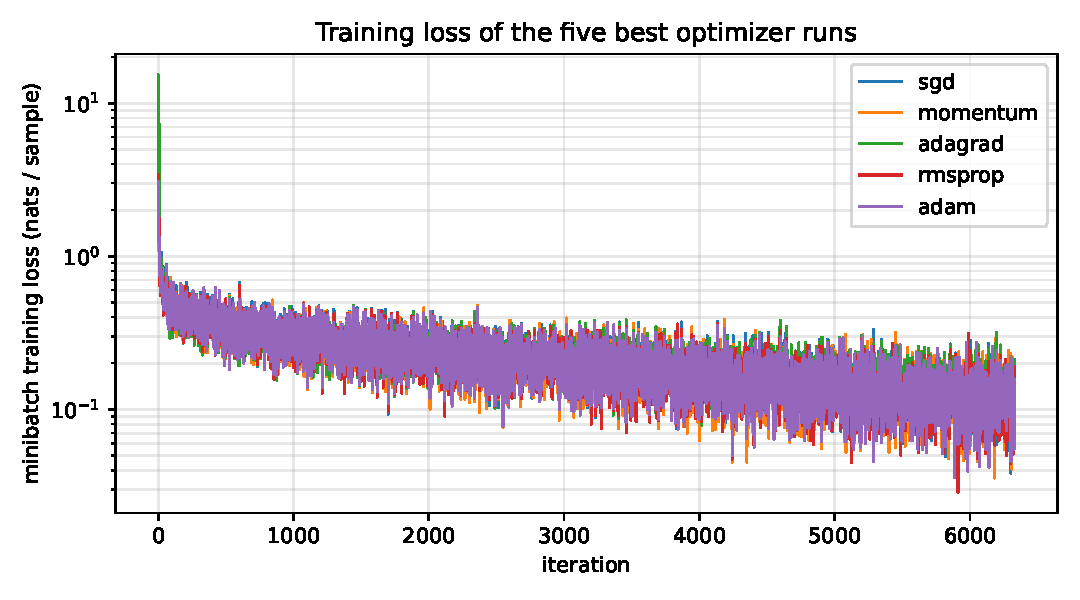
\includegraphics[width=0.95\textwidth]{p4_train_loss.pdf}
\caption{Minibatch training loss vs.\ iteration (log scale) for the
validation-best run of each optimizer.}
\end{figure}

\begin{figure}[ht]
\centering
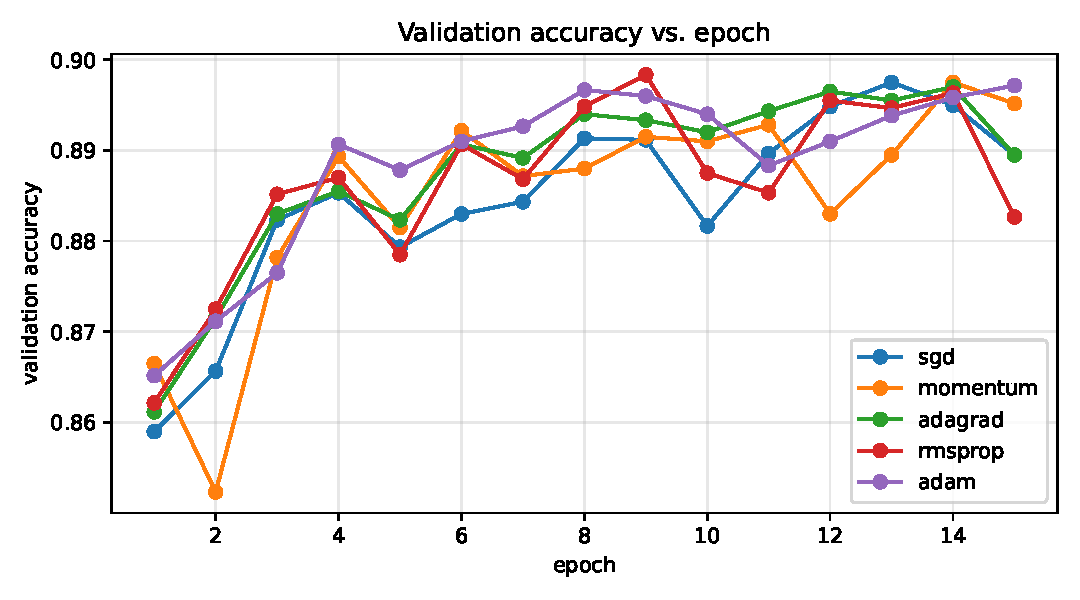
\includegraphics[width=0.8\textwidth]{p4_val_acc.pdf}
\caption{Validation accuracy vs.\ epoch for the same five runs.}
\end{figure}

\paragraph{(i)}
Ranked by iterations to first hit 87\% val accuracy (eval every 25
steps): momentum (425), Adam (600), AdaGrad (650), RMSProp (675),
SGD (875). Momentum gets there about \(2\times\) faster than SGD.

\paragraph{(ii)}
\begin{figure}[ht]
\centering
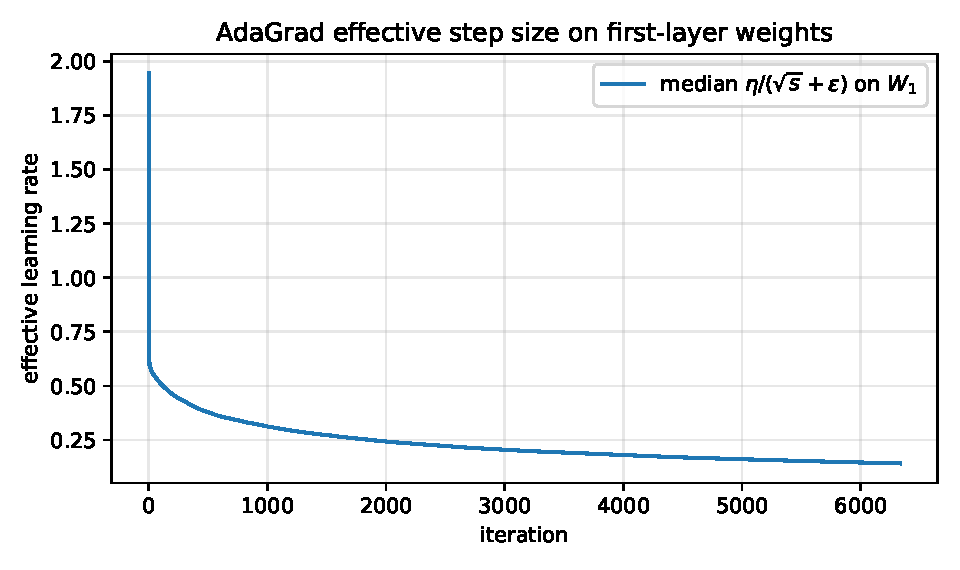
\includegraphics[width=0.75\textwidth]{p4_adagrad_lr.pdf}
\caption{Median effective learning rate
\(\eta/(\sqrt{s}+\epsilon)\) over the first-layer weights, AdaGrad.}
\end{figure}
AdaGrad's accumulator never forgets, so the effective step monotonically
shrinks [M3:80]. The plot does exactly that: after a short transient
the median \(\eta/(\sqrt{s}+\epsilon)\) on \(\mat{W}_1\) decays for
the rest of training. That is the failure mode --- late iterations
are taking tiny steps even though the loss is not done.

\paragraph{(iii)}
Best momentum \(\eta=0.03\), best SGD \(\eta=0.1\). The ratio is
about \(3.3\times\), in the same direction as the terminal-velocity
argument on [M3:78] (effective step \(\eta/(1-\rho)=10\eta\), so
momentum should want a \(10\times\) smaller \(\eta\)). The grid
point \(\eta=0.01\) for momentum was almost as good (val 0.896 vs.\
0.898), so the \(10\times\) rule is the right order of magnitude even
if the discrete grid did not land on it exactly.

\subsection*{(c) Activations and depth}

\begin{figure}[ht]
\centering
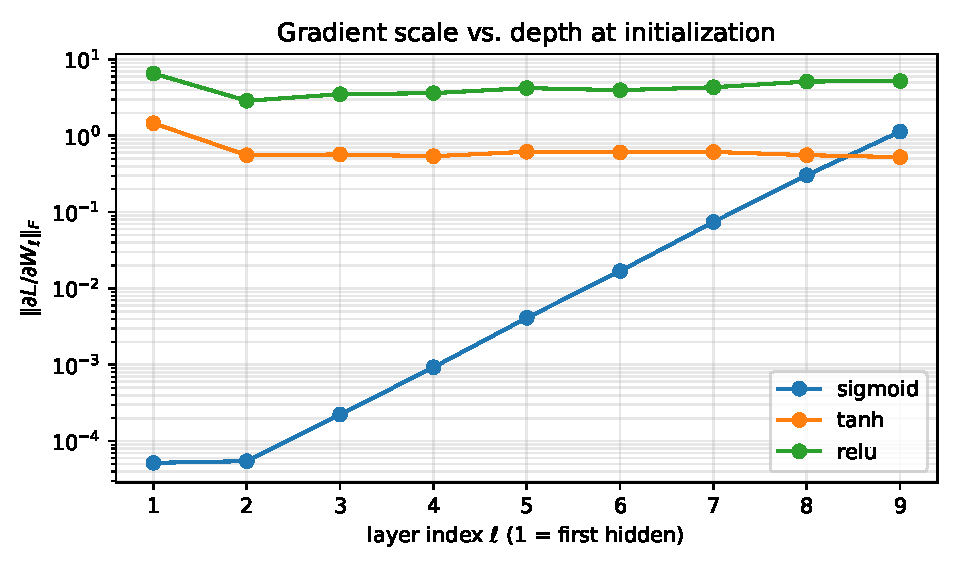
\includegraphics[width=0.75\textwidth]{p4_depth_gnorms.pdf}
\caption{Frobenius gradient norms \(\|\partial L/\partial W_\ell\|_F\)
on one minibatch at initialization, eight hidden layers of width 128.}
\end{figure}

Going backward from the output, the sigmoid gradient norm drops by
about \(0.24\times\) per hidden layer (geometric mean of
\(\|\partial L/\partial W_\ell\|_F/\|\partial L/\partial W_{\ell+1}\|_F\)).
That matches the bound \(\sigma'\le 0.25\) on [M3:43] almost exactly:
each VJP multiplies by at most \(1/4\), so eight hidden layers leave
the first-layer gradient at \(\sim 4^{-8}\approx 1.5\times 10^{-5}\)
times the last, which is what the plot shows
(\(5.2\times 10^{-5}\) vs.\ \(1.14\)).
Tanh and ReLU stay flat.

Test accuracies after 3 Adam epochs at \(\eta=10^{-3}\):
sigmoid \(0.7793\), tanh \(0.8591\), ReLU \(0.8607\).
Sigmoid still learns, even with those tiny early-layer gradients,
because Adam's update is \(\eta\,\hat m/(\sqrt{\hat v}+\epsilon)\).
As in Problem 2(d), the first step is \(\pm\eta\) regardless of
\(|g|\), and later steps normalize by the per-coordinate RMS, so a
systematically small gradient still moves. SGD would have stalled.

ReLU dead-unit fraction (zero on every validation example), averaged
over the eight hidden layers: \(2.2\%\) at initialization,
\(4.6\%\) after training. Most of the deaths are in the last two
hidden layers (8.6\% \(\to\) 14.1\% in the last one). He init keeps
the early layers alive; depth plus a hard-zero nonlinearity still
kills a tail of units [M3:44].

\subsection*{(d) Batch size and the roofline}

\begin{figure}[ht]
\centering
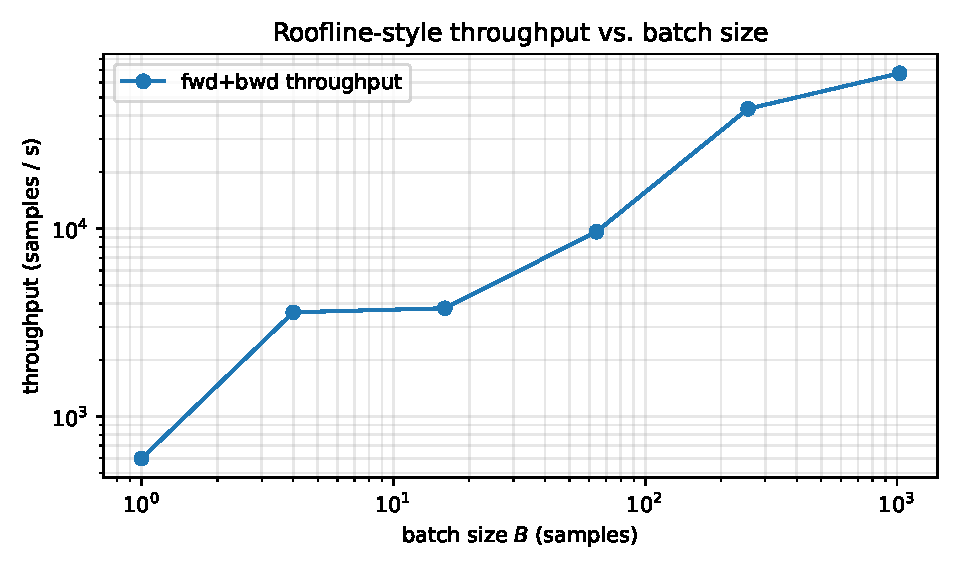
\includegraphics[width=0.75\textwidth]{p4_throughput.pdf}
\caption{Forward+backward throughput vs.\ batch size on this CPU
(log--log).}
\end{figure}

For one affine layer in FP32, reads of \(X,W\) and a write of \(Z\):
\[
I(B)
=\frac{B\,D_{\mathrm{in}}D_{\mathrm{out}}}
{2\bigl(B D_{\mathrm{in}}+D_{\mathrm{in}}D_{\mathrm{out}}+B D_{\mathrm{out}}\bigr)}
\ \text{FLOPs/byte}.
\]
First layer: \(I(1)=0.498\), \(I(128)=45.28\).
With \(I_{\mathrm{balance}}=40\), the first layer becomes
compute-bound at \(B\ge 108\). On this CPU the measured throughput
goes \(598\to 3.6\mathrm{k}\to 3.8\mathrm{k}\to 9.6\mathrm{k}\to 43.5\mathrm{k}\to 67.3\mathrm{k}\)
samples/s at \(B=1,4,16,64,256,1024\). It keeps climbing through the
small (memory-bound) batches and the slope eases after \(B\sim 256\),
past the \(B=108\) threshold [M3:75]. A CPU BLAS GEMM never becomes
as cleanly compute-bound as a systolic array, so the curve does not
fully flatten.

Output layer \(256\to 10\):
\[
\lim_{B\to\infty}I(B)
=\frac{D_{\mathrm{in}}D_{\mathrm{out}}}{2(D_{\mathrm{in}}+D_{\mathrm{out}})}
=\frac{2560}{532}=4.81<40.
\]
It can never become compute-bound. The matrix is short in \(D_{\mathrm{out}}\),
so even an infinite batch still streams more activation bytes than the
GEMM can hide. A batched network is not ``one compute-bound GEMM'';
the last layer stays memory-bound no matter how large \(B\) is.

\subsection*{(e) Memory planning and activation checkpointing}

At \(B=128\) in FP32:
weights \(535{,}818\times 4=2.143\) MB, gradients the same.
Optimizer state: SGD 0, momentum / AdaGrad / RMSProp 2.143 MB,
Adam 4.287 MB.
Activation cache: \(\mat{X}\) (\(401.4\) KB), \(\mat{H}_1\)
(\(262.1\) KB), \(\mat{H}_2\) (\(131.1\) KB), ReLU masks at 1 bit
(\(12.3\) KB), total \(806.9\) KB.
Each layer stashes its incoming activation for \(dW=X^\top\delta\)
and, if it has a ReLU, a 1-bit mask [M3:68].

Stashing only \(\mat{X}\) and recomputing both hidden activations
saves \(405.5\) KB at \(B=128\). Extra MACs are the two hidden
forwards, \(532{,}480\) / sample.
As a fraction of a full step that \emph{skips} first-layer
\(dX\), that is \(44.2\%\). If we also count \(dX\) (the 30\% quote
on [M3:70] is closer to ``backward \(\approx 2\times\) forward''),
it is \(33.2\%\). The gap is exactly the first-layer
\(\delta W^\top\) we said we can skip in (a).

\subsection*{(f) Quantizing the optimizer state}

\begin{figure}[ht]
\centering
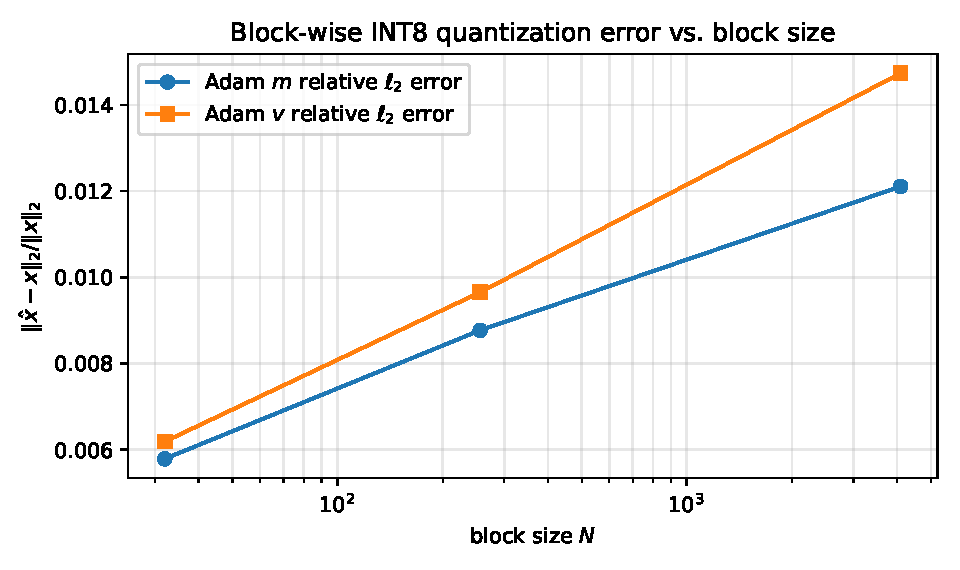
\includegraphics[width=0.75\textwidth]{p4_quant_error.pdf}
\caption{Relative \(\ell_2\) error of block-wise INT8 quantization of
the final Adam \(m\) and \(v\), vs.\ block size \(N\).}
\end{figure}

Mean relative \(\ell_2\) error, fraction of nonzero entries that
quantize to 0, and metadata (one FP32 scale per block):
\begin{center}
\begin{tabular}{lcccccc}
\toprule
 & \multicolumn{3}{c}{\(m\)} & \multicolumn{3}{c}{\(v\)} \\
\cmidrule(lr){2-4}\cmidrule(lr){5-7}
\(N\) & rel.\ err. & zero frac. & B/param & rel.\ err. & zero frac. & B/param \\
\midrule
32 & 0.0058 & 3.5\% & 0.125 & 0.0062 & 4.8\% & 0.125 \\
256 & 0.0088 & 5.0\% & 0.0156 & 0.0097 & 7.5\% & 0.0156 \\
4096 & 0.0121 & 6.8\% & 0.0010 & 0.0147 & 12.2\% & 0.0010 \\
tensor & 0.0157 & 8.0\% & \(4/n_i\) & 0.0193 & 14.0\% & \(4/n_i\) \\
\bottomrule
\end{tabular}
\end{center}

Larger blocks share one scale, so a single outlier inflates \(s\) and
the relative error grows. That is the ``one scale per block'' step of
[M3:95]: smaller groups keep the scale honest.

If a coordinate has \(\hat v=0\) but \(\hat m\neq 0\), the update
becomes \(\eta\hat m/\epsilon=10^8\eta\hat m\), i.e.\ a huge step.
At \(N=256\) already 7.5\% of the nonzero \(v\) entries collapse to
0; at one-scale-per-tensor it is 14\%. Linear INT8 is not safe for
\(v\). A non-linear / quantile map spends codes on the small \(v\)
values that actually matter for the \(1/\sqrt{v}\) denominator,
instead of letting them all collapse to 0.

\end{document}
